\documentclass[12pt,a4paper]{article}
\usepackage{graphicx} % Required for inserting images
\usepackage{tikz}
\usepackage[left=2.00cm, right=1.00cm]{geometry}
\usepackage{xcolor} % before tikz or tkz-euclide if necessary
\usepackage{amsmath}
\usepackage{siunitx}
\usepackage{chemfig}
\usetikzlibrary{calc}
\begin{document}
\begin{center}
    \large\textbf{Trykk fra faste stoffer mot en flate:}\\
\end{center}
Vi kan se på en firkantet kloss som ligger på et bord:\\\\\\\
\begin{center}
    \begin{tikzpicture}[scale=0.8]
        \draw (4,0)--(4,4);
        \draw (2,4)--(10,4);
        \draw (8,0)--(8,4);
        \draw (5,4) rectangle (7,6);
    \end{tikzpicture}    
\end{center}
Denne klossen har en masse (4,3 kg) og et areal som berører bordplaten.  Den yter dermedet trykk P mot bordet.  Sidene er lengde lik 40cm, høyde lik 10cm og bredde lik 20cm:\\
\begin{tikzpicture}[scale=1.5,transform canvas={shift={(6cm,-3cm)}}]


% Dimensjoner
\def\L{4}   % lengde
\def\B{2}   % bredde (dybde)
\def\H{1}   % høyde

% Vektor for dybde (perspektiv)
\coordinate (D) at (-0.5,0.3);

% Bunnflate
\draw (0,0) -- (\L,0) -- ++(D) -- ++(-\L,0) -- cycle;

% Vertikale kanter (høyde)
\draw (0,0) -- ++(0,\H);
\draw (\L,0) -- ++(0,\H);
\draw ($(0,0)+ (D)$) -- ++(0,\H);
\draw ($( \L,0) + (D)$) -- ++(0,\H);

% Toppflate
\draw (0,\H) -- (\L,\H) -- ++(D) -- ++(-\L,0) -- cycle;

% Linjer bakover (dybde)
\draw (\L,0) -- ++(D);
\draw (\L,\H) -- ++(D);
\node at (2,1.5) {lengde=40cm};
\node at (4.8,0.5) {høyde=10cm};
\node at (-1.4,0.2) {bredde=20cm};
\end{tikzpicture}\\
\vspace{4cm}
\\Denne klossen kan plasseres på tre forskjellig måter på bordet.  Og de vil gi ulikt trykke mot bordet. For arealet vil variere.  Vi beregner arealene, og gjør om til meter:\\
areal 1: lengde 40cm, bredde 10cm:  $A_1=0,4m\cdot 0,1m=0,04m^2$\\
areal 2: lengde 40cm, bredde 20cm:  $A_1=0,4m\cdot 0,2m=0,08m^2$\\
areal 3: lengde 20cm, bredde 10cm:  $A_1=0,2m\cdot 0,1m=0,02m^2$\\
Vi er nå klare for å beregne de 3 trtyhkkene  Vi tar da utgangspunkti definisjonen for trykk:
$$P=\frac{F}{A}$$
der:\\
P=trykk ($N/m^2, Pa (Pascal)$\\
F=kraft (N, Newton)\\
A=Areal ($m^2$)\\
\newpage
\noindent Kraften vi skal finne her  er lik tyngdekraften $G=m\cdot g$\\  
her er:\\
G=Tyngdekraften (N)\\
m=klossens masse (kg)\\
g=tyngdens akselerasjon ($N/m^2$)\\\\
\noindent Vi beregner trykkene nå når massen til klossen er 3kg:\\
$$P_1=\frac{G}{A_1}=\frac{3kg\cdot 9,8m/s^2}{0,04m^2}=735N/m^2$$\\
$$P_2=\frac{G}{A_2}=\frac{3kg\cdot 9,8m/s^2}{0,08m^2}=367,5N/m^2$$\\
$$P_3=\frac{G}{A_3}=\frac{3kg\cdot 9,8m/s^2}{0,02m^2}=1470N/m^2$$\\\\
Var resultatet overraskende for deg? At trykket blir større når arealet blir mindre? Årsaken er jo at når du "deler" et tall på et tall som er mindre, så blir brøken større enn telleren. Prøv å del 1 på 0,5.  Du får svaret 2.
\begin{center}
    \large\textbf{Trykk i væsker:}\\
\end{center}
Når iv har en tank med en væske så vil trykektr øke når man går nedover i væsken.  Dette fordi man da får en væske over seg som yter et trykk mot flaten.  Trykkendringen kan beregnes etter følgende formel:
$$\Delta P =\rho\cdot g \cdot h$$
der:\\
$\Delta P=trykkendring (N/m^2)$\\
$\rho=væskens tetthet, kg/m^3.$ For vann: $\rho=1000kg/m^3$\\
h=væskens høyde i tanken (m)
\newpage
\begin{center}
    \large\textbf{Arbeidsoppgave om trykk:}
\end{center}\vspace{1cm}

\noindent 1.	Hvordan defineres begrepet trykk? Hint:$F=G=m\cdot g \hspace{1.2cm} g=9,8m/s^2$\\

\noindent 2. En murstein på 3kg har lengde 25cm, høyde 5cm og bredde 10cm.  Beregn hvordan trykket endrer seg  når vi legger steinen på et gulv.   Når er trykket størst?\\\\
3. Beregn trykkendringen i en tank med høyde 30m. Hint: $\Delta P=\rho_{vann} \cdot g\cdot h\hspace{1.20cm} \rho_{vann}=1000kg/m^3$\\\\

\noindent 4. I en tank viser trykktransmitteren en trykkforskjell på 100kPa.  Hvor høyt står væsken i tanken?\\\\

\noindent 5. Inne i tanken er det montert en sikkerhetsventil som er formet som et stempel som er koblet til en fjær.  Stempelet vil åpne når trykket i  tanken er over 20bar.   Hvor stor er kraften mot fjæra da når stempelet har en diameter på 5cm?\\\\
\noindent 6.	Om vi ønsket å bytte ut fjæra med en stein, hvor tung måtte steinen være da? (Hint: F=G=m*g)\\\\

\noindent 7.	Vi har gitt følgende stempel med en gass som er innestengt.  Vi har et stempel som vi kan skyve inn og ut:\vspace{0.5cm}\\
\begin{center}
    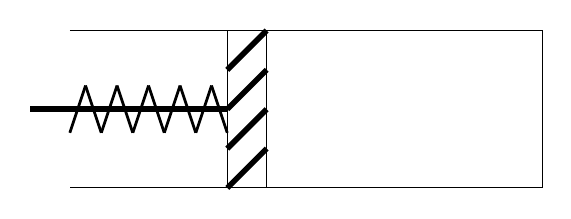
\begin{tikzpicture}
        %stempel med variabel
        \pgfmathsetmacro{\myLength}{4}
        \draw (2,2)--(8,2)--(8,0)--(2,0);
        \draw (\myLength,0)--(\myLength+0.5,0)--(\myLength+0.5,2)--(\myLength,2)--(\myLength,0);
        \draw [line width=2pt] (\myLength,0)--(\myLength+0.5,0.5);
        \draw [line width=2pt] (\myLength,0.5)--(\myLength+0.5,1);
        \draw [line width=2pt] (\myLength,1)--(\myLength+0.5,1.5);
        \draw [line width=2pt] (\myLength,1.5)--(\myLength+0.5,2);
        \draw [line width=2pt] (\myLength,1)--(\myLength-2.5,1);
        \draw [line width=1pt] (2,0.7)--(2.2,1.3);
        \draw [line width=1pt] (2.2,1.3)--(2.4,0.7);
        \draw [line width=1pt] (2.4,0.7)--(2.6,1.3);
        \draw [line width=1pt] (2.6,1.3)--(2.8,0.7);
        \draw [line width=1pt] (2.8,0.7)--(3.0,1.3);
        \draw [line width=1pt] (3.0,1.3)--(3.2,0.7);
        \draw [line width=1pt] (3.2,0.7)--(3.4,1.3);
        \draw [line width=1pt] (3.4,1.3)--(3.6,0.7);
        \draw [line width=1pt] (3.6,0.7)--(3.8,1.3);
        \draw [line width=1pt] (3.8,1.3)--(4.0,0.7);
    \end{tikzpicture}
\end{center}\vspace{1cm}
For øyeblikket er temperaturen 300C, V=3,6L og trykket er 1bar.  Vi trykker stempelet innover til volumet er 0,72L.   Vi antar at temperaturen er konstant.  Hvor stort blir det nye trykket?
\\\\8.	Vi varmer opp beholderen til 800C .  Stempelet beveger seg utover.  Hvor langt utover beveger stempelet seg når vi antar at trykket er konstant?\\


\end{document}